\documentclass[12pt,a4paper]{article}
\usepackage[utf8]{inputenc}
\usepackage{amsmath}
\usepackage{amsfonts}
\usepackage{amssymb}
\usepackage{hyperref}
\usepackage{graphicx}
\usepackage[a4paper]{geometry}
\usepackage{fullpage}
\newcommand{\unit}[1]{\ensuremath{\, \mathrm{#1}}}
\author{Gergely Imreh}
\title{Zeeman slower summary}
\date{\today, v2}
\begin{document}

\maketitle

\section{Introduction}

The purpose of this document to summarize our simulation and construction results of the Zeeman slower in our lab.

\section{Theory}

\subsection{Field shape}

\begin{equation}
a(z) = -\frac{\hbar k \Gamma}{2 m} \frac{s}{1 + s + 4 \delta(z)^2 / \Gamma^2}
\label{eq:accel}
\end{equation}
where $s$ is $I/I_{\rm sat}$ saturation parameter. The assumed maximum deceleration is at $s \rightarrow \infty$, and at $\delta = 0$ we have $\eta = \frac{s}{1 + s}$.

The detuning is 
\begin{equation}
\delta(z) = k v(z) + \Delta - \frac{\mu'}{\hbar} B(z)
\end{equation}
where 
\begin{equation}
\mu' = \mu_{B}(g_e m_e - g_g m_g)
\end{equation}
and in our case $\mu' = \mu_{B}$.

Most people use the ``ideal'' field profile, assuming constant deceleration (e.g adapted from \cite{Bell2010}):
\begin{equation}
B_{\rm ideal}(z) = \frac{\hbar k}{\mu'}\sqrt{v_0^2 + 2 \eta a_m z} + B_a
\label{eq:bideal}
\end{equation}
where $\eta$ is the cooling efficiency, $v_0$ is the maximum capture velocity chosen (or fixed by a given slower length and $\eta$), $a_m = -\frac{\hbar k \Gamma}{2 m}$ is the maximum deceleration, from Eq. \ref{eq:accel} setting $s = \infty$, and $B_a$ is a bias field, or an equivalent laser detuning from the resonance as $B_a = \frac{\hbar}{\mu'} \Delta$.

In this case the magnetic field gradient is
\begin{equation}
\frac{\partial B_{\rm ideal}}{\partial z} = \frac{\hbar k}{\mu'} \frac{\eta a_m}{\sqrt{v_0^2 + 2 \eta a z}}
\end{equation}
which is a negative number because $a_m < 0$.

From Eq. \ref{eq:accel} and \ref{eq:bideal} one can deduce that the efficiency is
\begin{equation}
\eta = \frac{s}{1 + s}
\end{equation}

\subsection{Detuning}

The detuning at a given position is given by three contribution as
\begin{equation}
\delta = k v + \Delta - \frac{\mu'}{\hbar} B
\end{equation}
where v is the atomic velocity.

\begin{equation}
\frac{\partial \delta}{\partial z} = k \frac{\partial v}{\partial z} - \frac{\mu'}{\hbar}\frac{\partial B}{\partial z} = k \frac{\partial v}{\partial t} \frac{1} {\frac{\partial z}{\partial t}} - \frac{\mu'}{\hbar}\frac{\partial B}{\partial z}
= k \frac {a}{v} - \frac{\mu'}{\hbar}\frac{\partial B}{\partial z}
\label{eq:dddz}
\end{equation}

Without change in the magnetic field (that is zero gradient), there's always just going to lower detuning. On the other hand, when there's $\partial B/\partial z < 0$: the can be stable and unstable points: either 1 stable and 2 unstable, or 1 unstable if $|\partial B / \partial z| >> 0$ (set a more correct level for this).


Figure \ref{fig:dddz1} shows the spatial gradient of the detuning $\partial \delta / \partial z$ for a set of commonly used parameters and assuming a constant magnetic field. The gradient is negative in the entire region, meaning that the detuning is moving to the red. Given the parameters, that means $\partial v / \partial z < 0$, which is deceleration. Given the profile, the deceleration is the largest near the resonance, and away from it is decreasing rapidly.

\begin{figure}[htb]
\centering
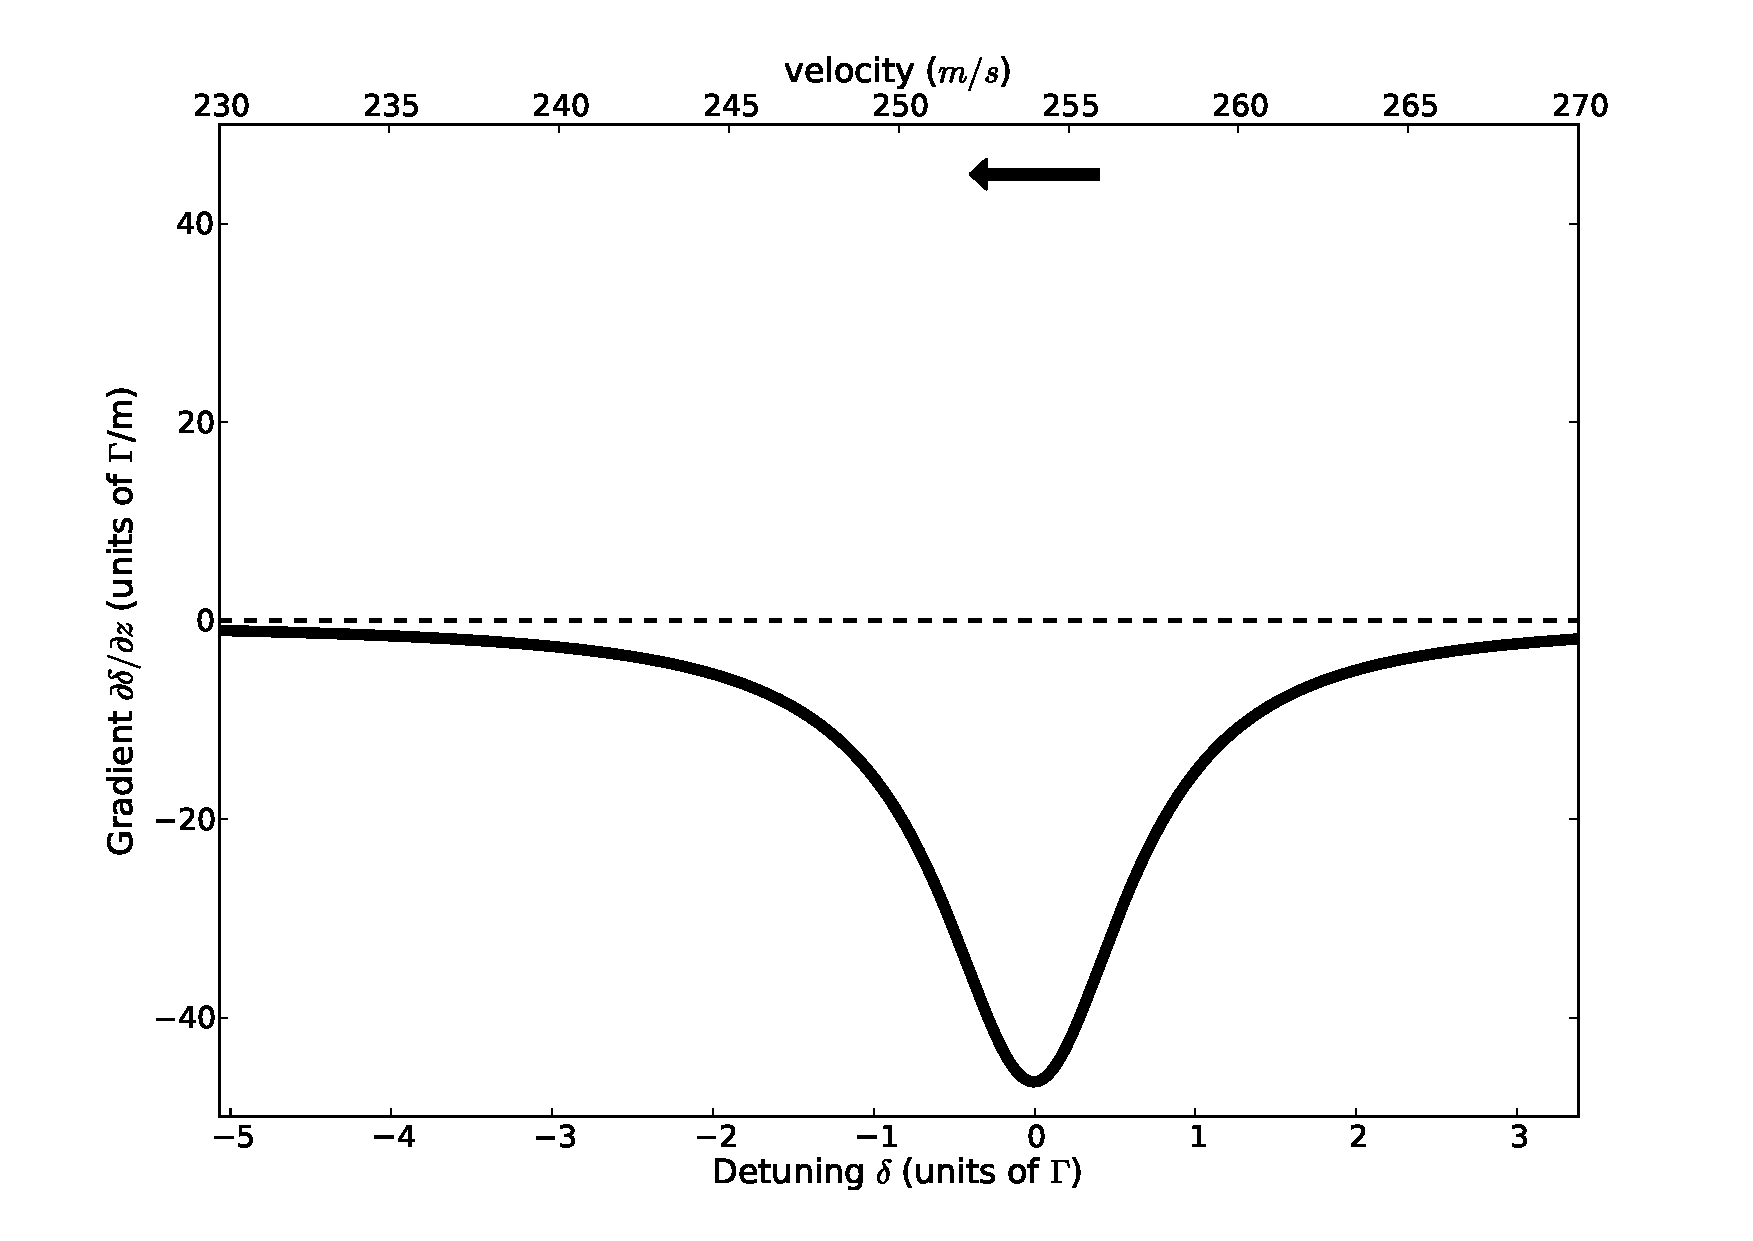
\includegraphics[width=1.0\textwidth]{detu1}
\caption{The spatial gradient of detuning $\delta$ with $\partial B/\partial z=0$ at $z=0$, $v_0 = 254~m/s$, $\eta = 0.5$ and $s = 1$. The arrow means that over the whole whole plotted range, the detuning is decreasing (going red).}
\label{fig:dddz1}
\end{figure}

Figure \ref{fig:dddz2} is a similar plot using the same parameters except for the magnetic field, where $B_{\rm ideal}$ is used as defined in Eq. \ref{eq:bideal}, with its field gradient. Now $\partial \delta / \partial z \geq 0$, meaning the detuning is moving to the blue (because of the change in $B$). There's one special point (for the given parameters) near $\delta = 0$ where $\partial \delta / \partial z = 0$, that is the detuning will be constant. Since $B$ is changing, this implies change in $v$ as well, and given the signs of the changes, implies deceleration.

\begin{figure}[htb]
\centering
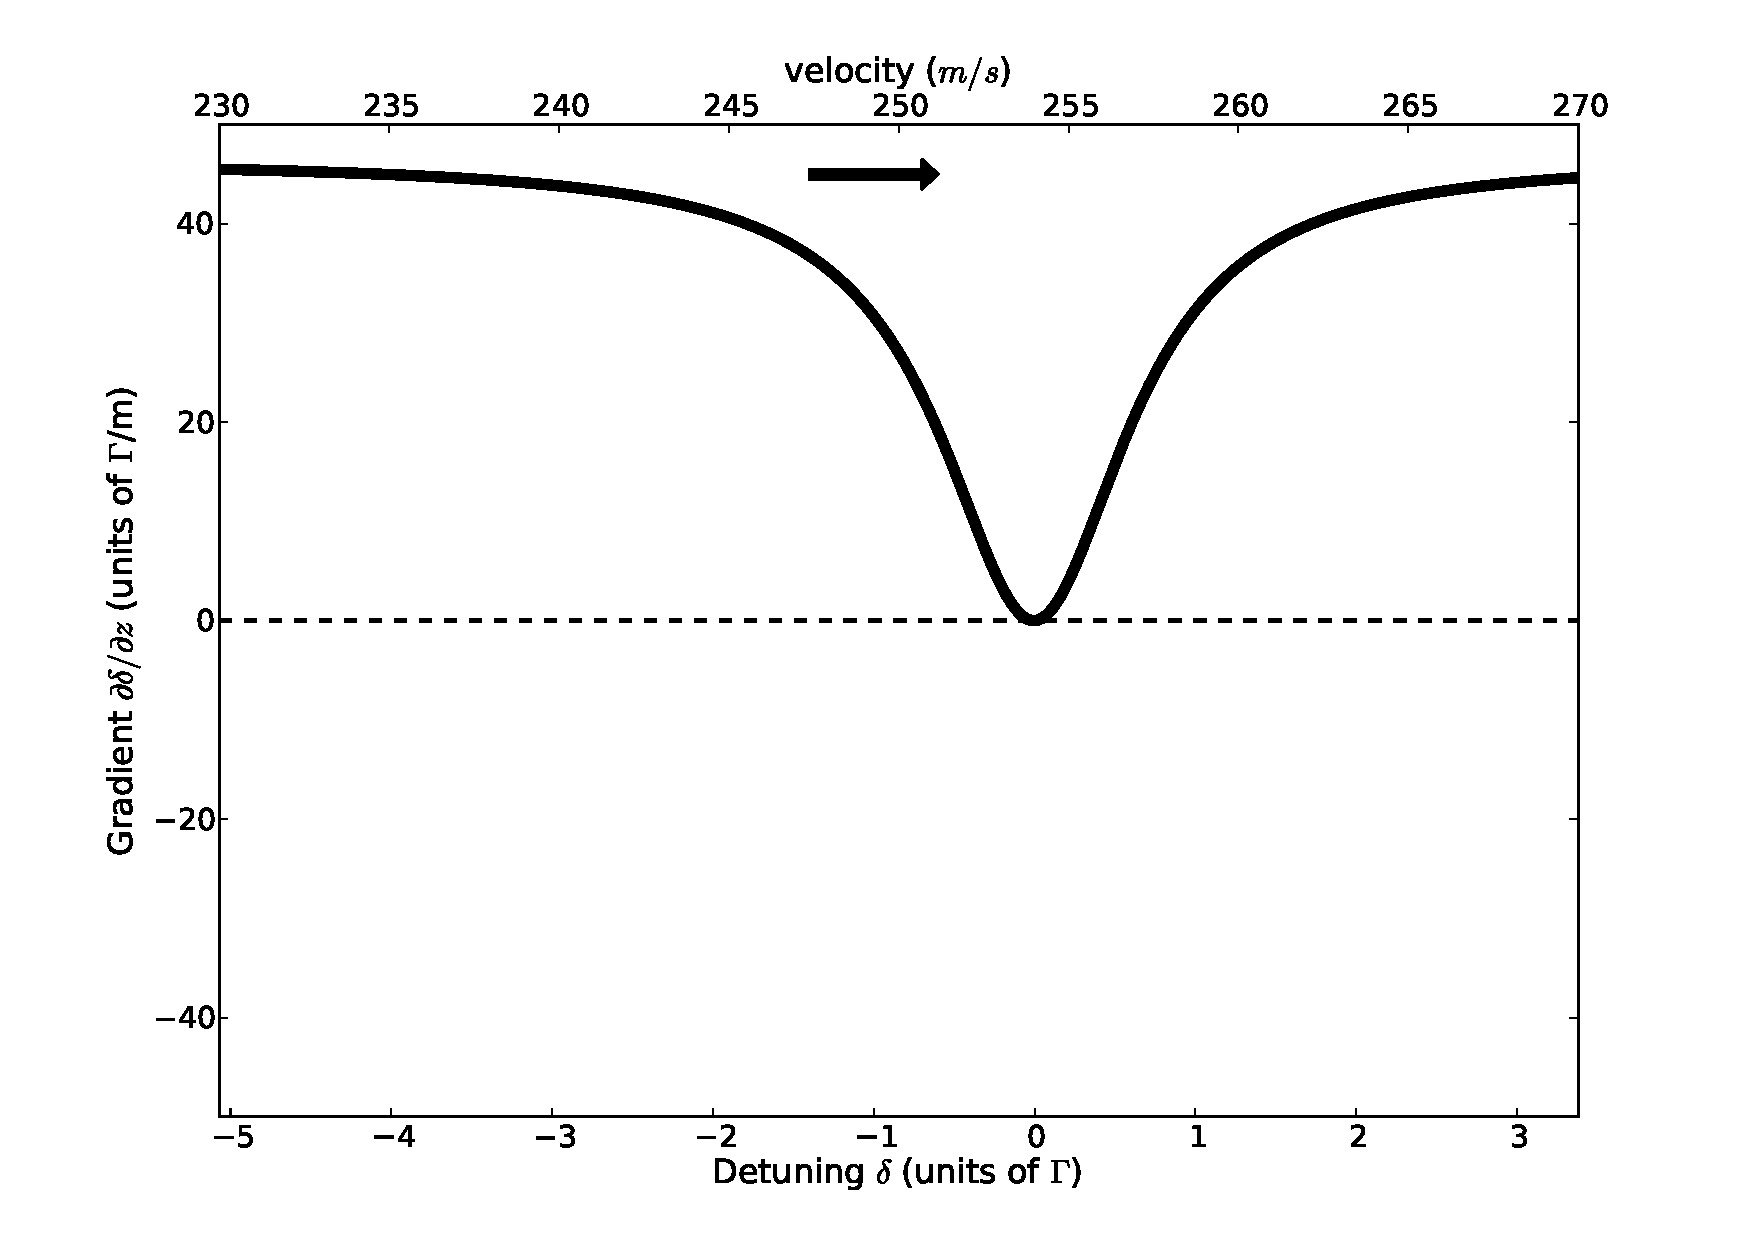
\includegraphics[width=1.0\textwidth]{detu2}
\caption{As Fig. \ref{fig:dddz1} but with $B=B_{\rm ideal}$. The arrow means that over the whole range the detuning is increasing (going blue). Exception is near $\delta = 0$ where there is a fixed point.}
\label{fig:dddz2}
\end{figure}

\begin{figure}[htb]
\centering
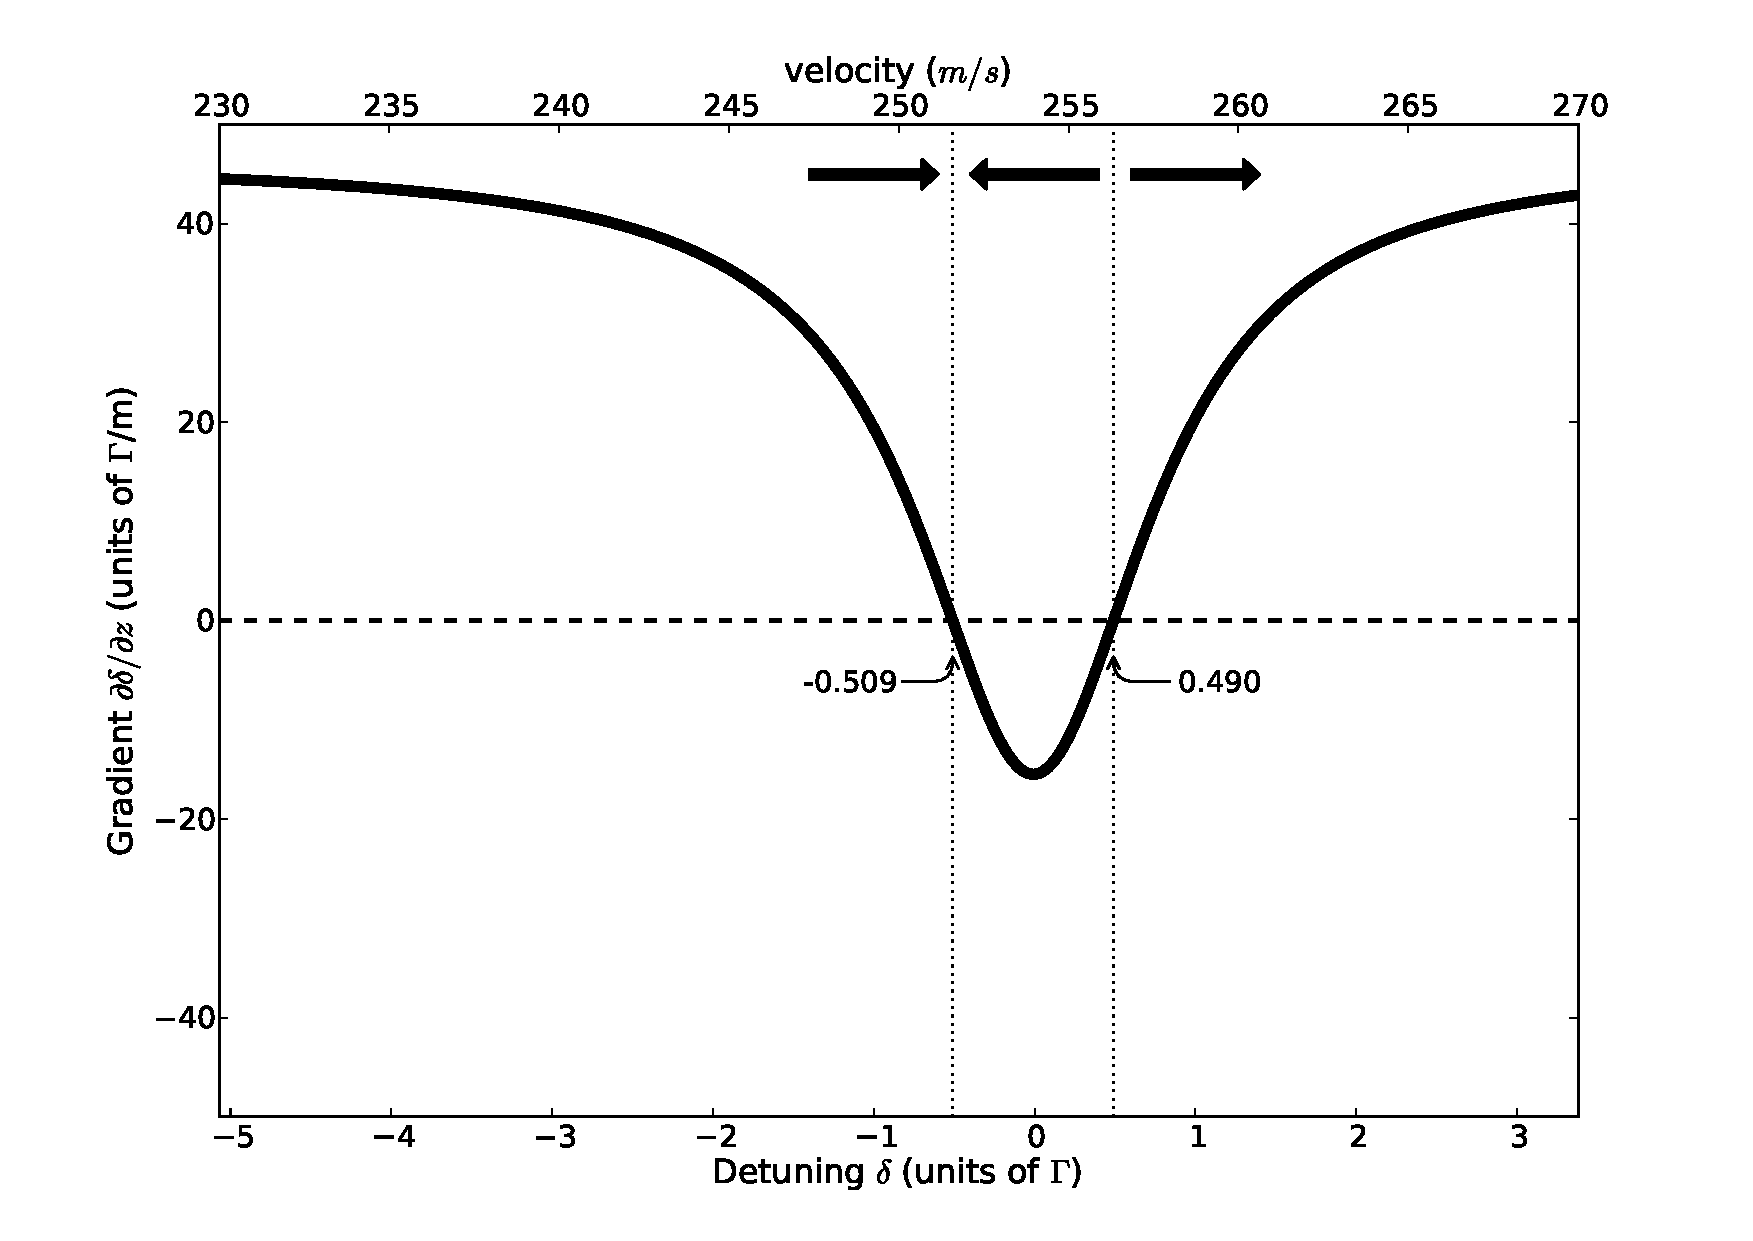
\includegraphics[width=1.0\textwidth]{detu3}
\caption{As Fig. \ref{fig:dddz2} but with $s = 2$, which means higher laser intensity. The line is widened and its height has increased. Now there is a true stable fixed point near $\delta = -0.5 \Gamma$ and an unstable fix point near $\delta = 0.5 \Gamma$. Further increase of laser intensity will push the fixed points away from $\delta = 0$.}
\label{fig:dddz3}
\end{figure}

The zero crossing can be calculated analytically by reorganizing Equation \ref{eq:dddz}. We can make the following substitutions for notational convenience:
\begin{eqnarray}
v &=& \frac{1}{k}\left(\delta - \Delta + \frac{\mu'}{\hbar}B\right) \\
A &=& \frac{\mu'}{\hbar}B \\
X &=& A - \Delta \\
Y &=& 1+s \\
Z &=& \frac{4}{\Gamma^2} \\
W &=& - \frac{\hbar k^3 \Gamma s}{2 m}.
\end{eqnarray}
The detuning $\delta$ can then be expressed as
\begin{equation}
\delta^3 + X \delta^2 + \frac{Y}{z} \delta + \frac{A X Y - W}{A Z}= 0
\label{eq:deltacubic}
\end{equation}
which is just a standard cubic equation. The displayed 2 roots (out of the 3) of Figure \ref{fig:dddz3} were calculated with this method.

\subsection{Controlling the final velocity}

The final velocity depends on multiple parameters. We can choose a velocity that we can design for, effectively making a shorter slower on the ``slow side''. In practice the current in the negative coil can be adjusted to directly affect the final velocity. Other groups usually reduce the current in the negative coil. The Doppler cooling beam's saturation parameter also affects the final velocity, as higher saturation will give rise to larger red detuning $\delta \ll 0$, and thus lower final velocity.

Some relevat simulations are shown in Figures \ref{fig:trajectory1}, \ref{fig:trajectory2} and \ref{fig:trajectory3} in Section \ref{seq:sim}. The magnetic field is the same as our slower, saturation parameter $s=2$, and the three cases have final velocities $22\unit{m/s}$, $76\unit{m/s}$ and $101\unit{m/s}$, respectively. These values should be available by solving Equation \ref{eq:deltacubic} for the minimal velocity, but that has not been tested yet.

\subsection{Transverse cooling}

Other groups are doing transverse cooling to reduce the transverse spread of atomic velocities, thus providing larger flux into the experimental area. For this we have avalailable windows on the double-cube sections before and after the slower. Some group is using optical molasses on the slow end of the slower  near the area with the largest negative field \cite{Joffe1993}, while others do transverse collimation and molasses on the fast end of the slower \cite{Slowe2005}.


\section{Construction}

\subsection{Simulation}
\label{seq:sim}

Here are the simulation results, and our choice for the used design. 
Finally a $0.59\unit{m}$ slower length was chosen, with AWG12 teflon coated wire, and maxium layer number of 10. The simulated layer positions are listed in Table \ref{tab:layers}, while the field is plotted in Figure \ref{fig:simcoil}.

\begin{table}[htb]
\begin{center}
\begin{tabular}{|c|c|c|c|}
\hline 
\textbf{Layer\#} & \textbf{Turns} & \textbf{Start (mm)} & \textbf{End (mm)} \\ 
\hline 
9 & 18 & -23.9 & 13.9 \\ 
\hline 
7 & 31 & 13.9 & 79.0 \\ 
\hline 
6 & 31 & 79.0 & 144.1 \\ 
\hline 
5 & 30 & 144.1 & 207.1 \\ 
\hline 
4 & 27 & 207.1 & 263.8 \\ 
\hline 
3 & 26 & 263.8 & 318.4 \\ 
\hline 
2 & 23 & 318.4 & 366.7 \\ 
\hline 
1 & 21 & 366.7 & 410.8 \\ 
\hline 
0 & 19 & 410.8 & 450.7 \\ 
\hline 
1 & 17 & 450.7 & 486.4 \\ 
\hline 
2 & 15 & 486.4 & 517.9 \\ 
\hline 
3 & 12 & 517.9 & 543.1 \\ 
\hline 
4 & 18 & 543.1 & 580.9 \\ 
\hline 
8 & 2 & 580.9 & 585.1 \\ 
\hline 
10 & 11 & 585.1 & 608.2 \\ 
\hline 
\end{tabular} 
\end{center}
\caption{Zeeman slower winding data}
\label{tab:layers}
\end{table}


\begin{figure}[htb]
\centering
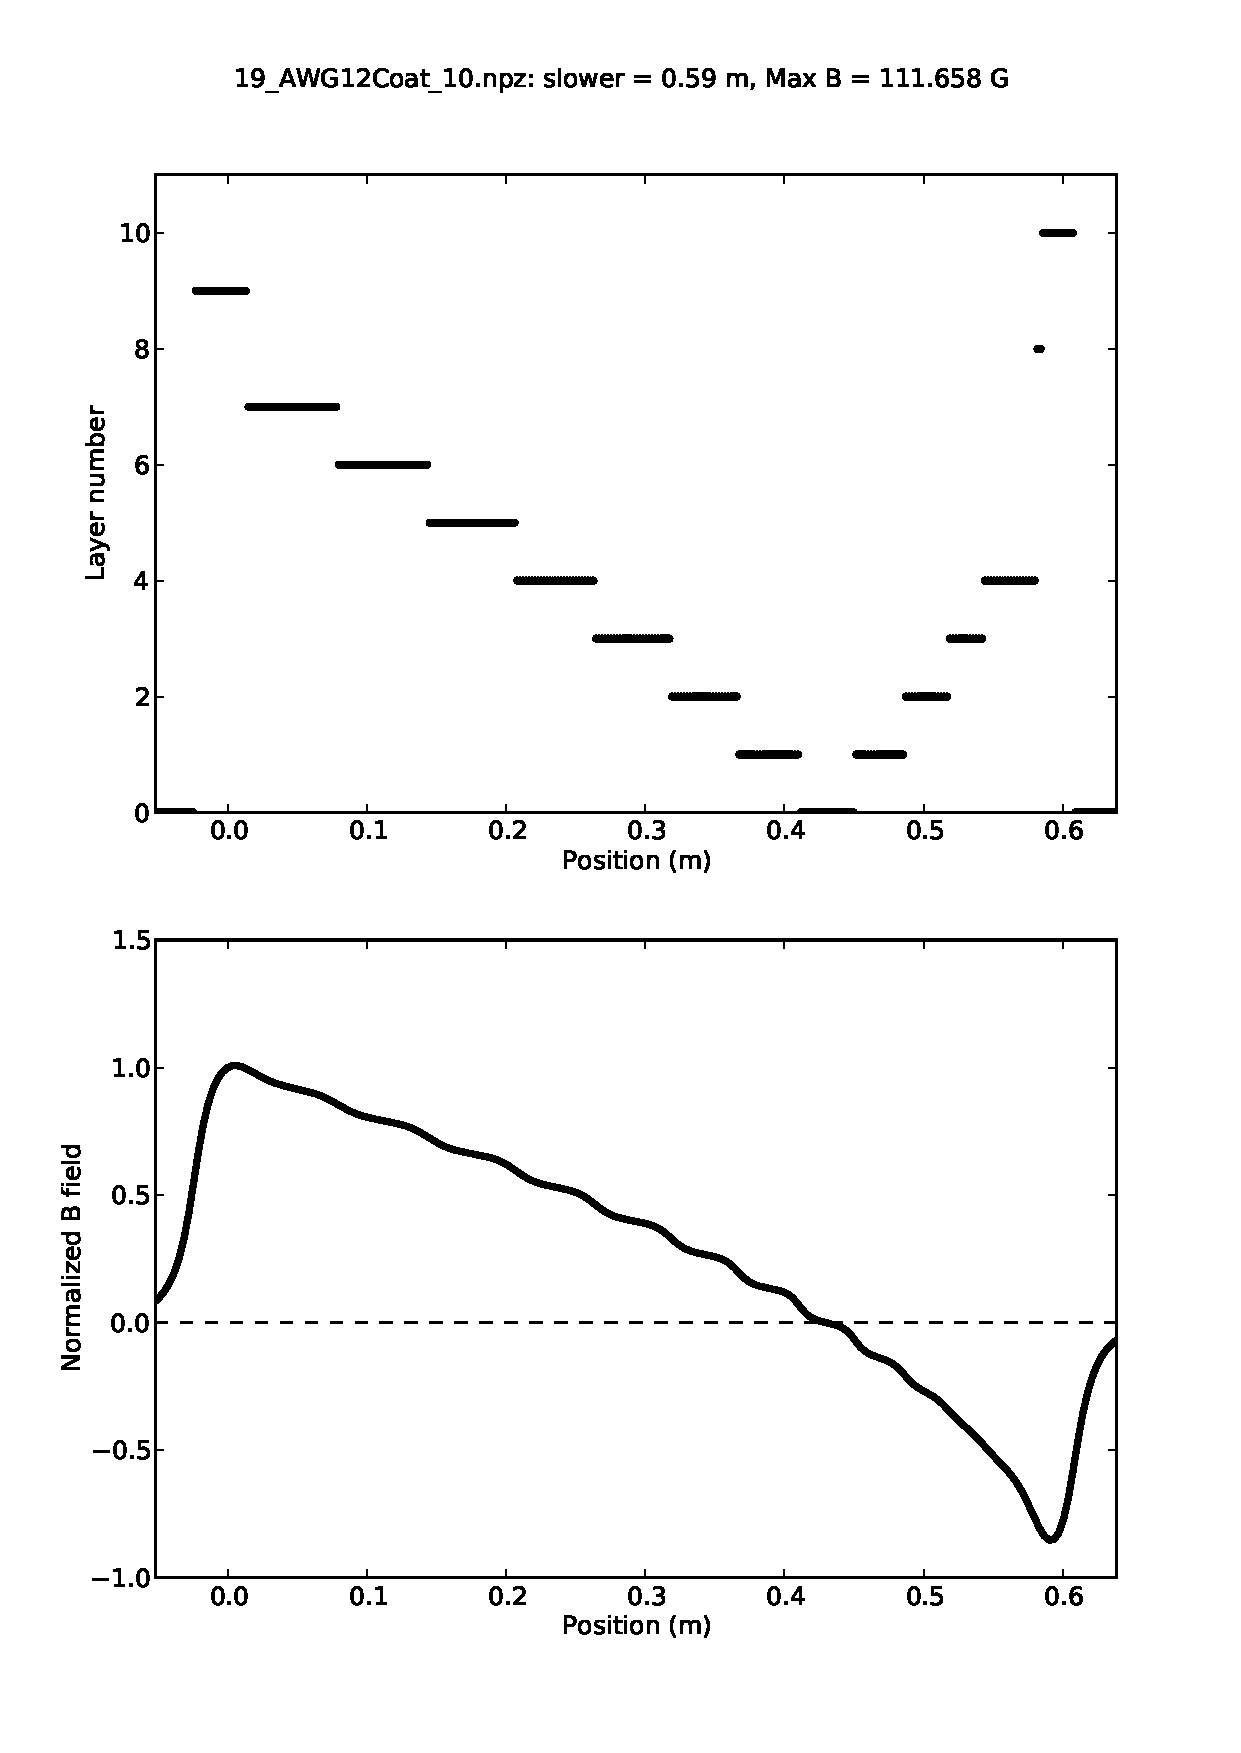
\includegraphics[width=1.0\textwidth]{19_AWG12Coat_10}
\caption{Results of coil somulation, layer numbers and field profile. The effective length is $0.59\unit{m}$, the winded coil length is $\approx0.63\unit{m}$ }
\label{fig:simcoil}
\end{figure}

There's also simulation results for the the effect of reduced current in the negative coil. That seems to be the standard method for adjusting the flux, though the reduction is not as severe as we simulated. The reduction seems to be more in the 0.9-0.8 region compared to the designed current, when it is the same value on both coils: $I_{pos} = I_{neg}$. Figure \ref{fig:trajectory1} shows the simulated atom trajectories (the velocity as a function of position along the slower) for the designed current, while Figure \ref{fig:trajectory2} shows $I_{pos} = 0.5 \times I_{neg}$ and Figure \ref{fig:trajectory3} the extreme $I_{pos} = 0.25 \times I_{neg}$.


\begin{figure}[htb]
\centering
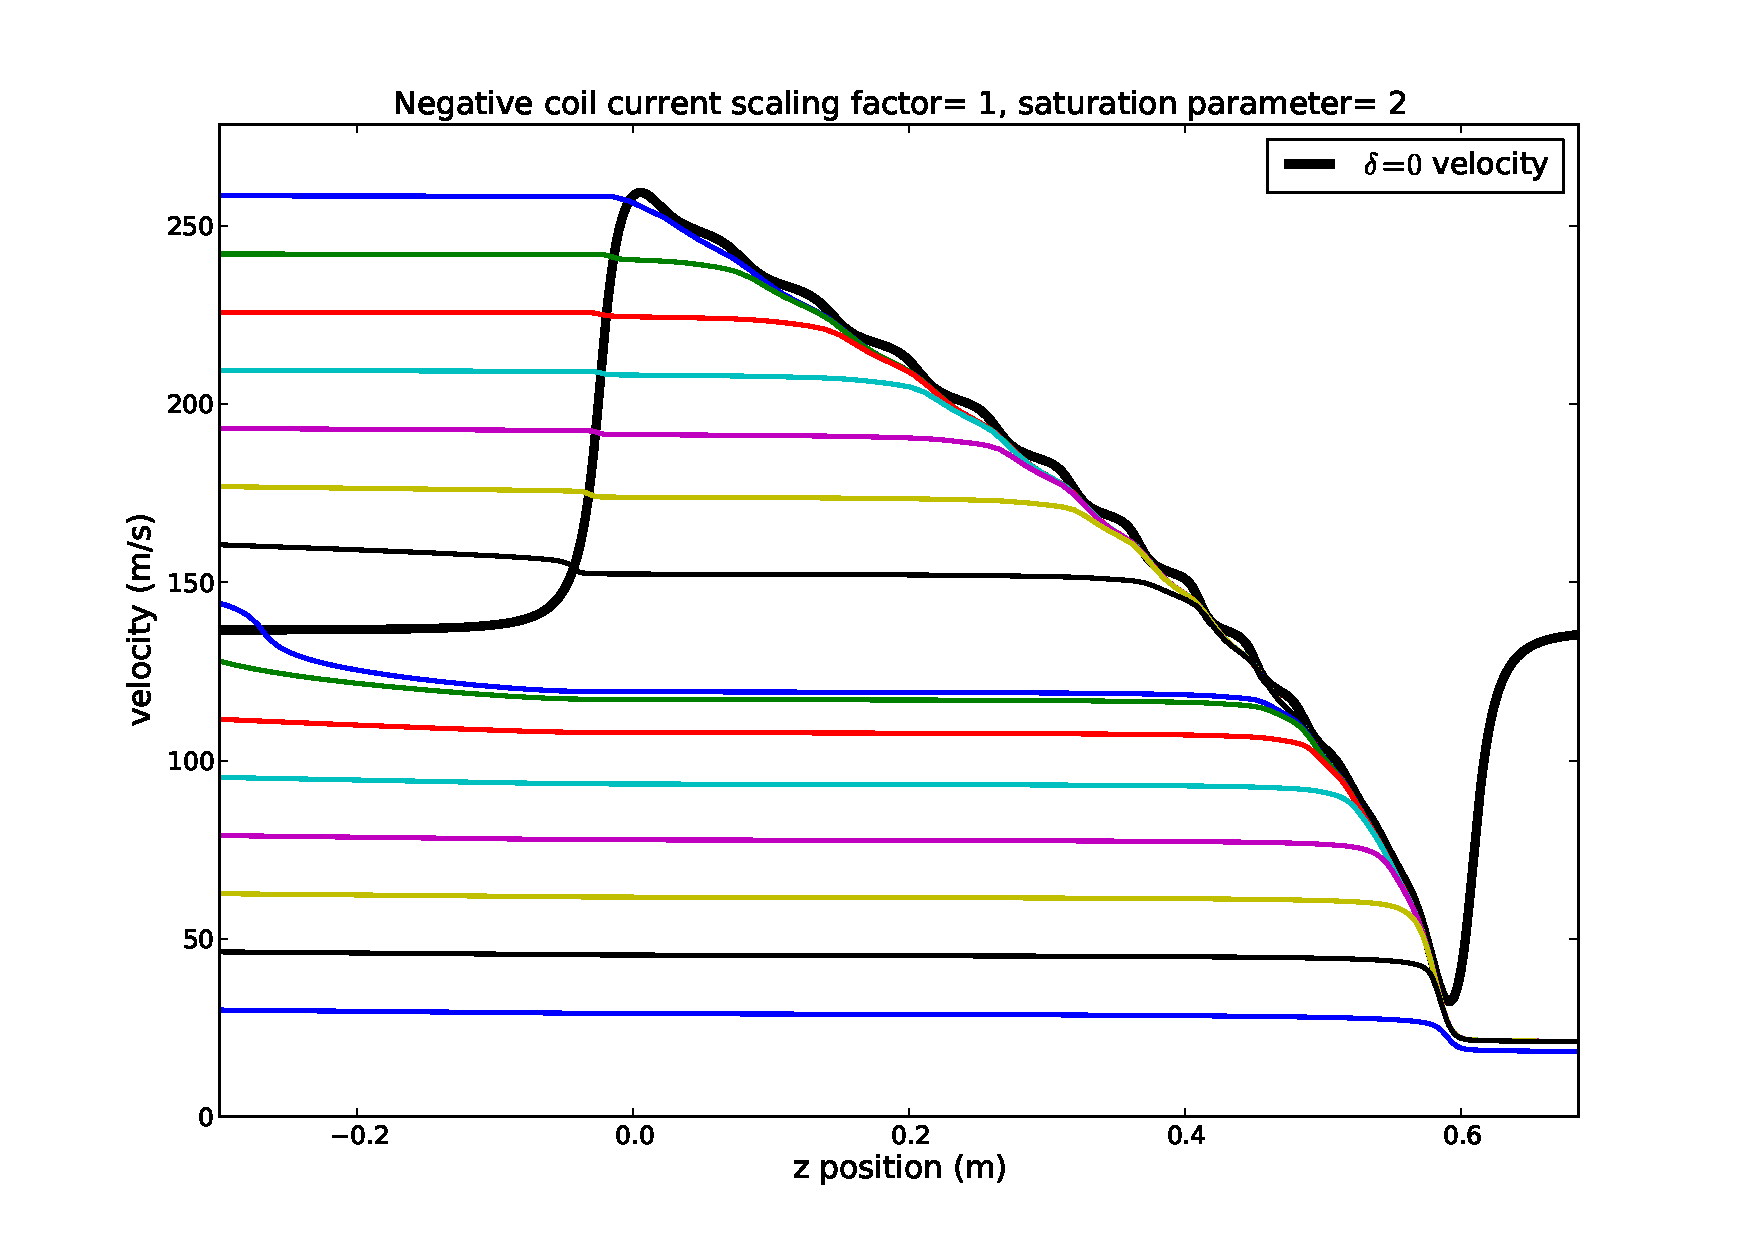
\includegraphics[width=0.9\textwidth]{trajectory03_1}
\caption{Atomic trajectories of different starting velocities, with the designed currents for both coils. Simulation is done by solving the differential equations of motion for the velocity.}
\label{fig:trajectory1}
\end{figure}

\begin{figure}[htb]
\centering
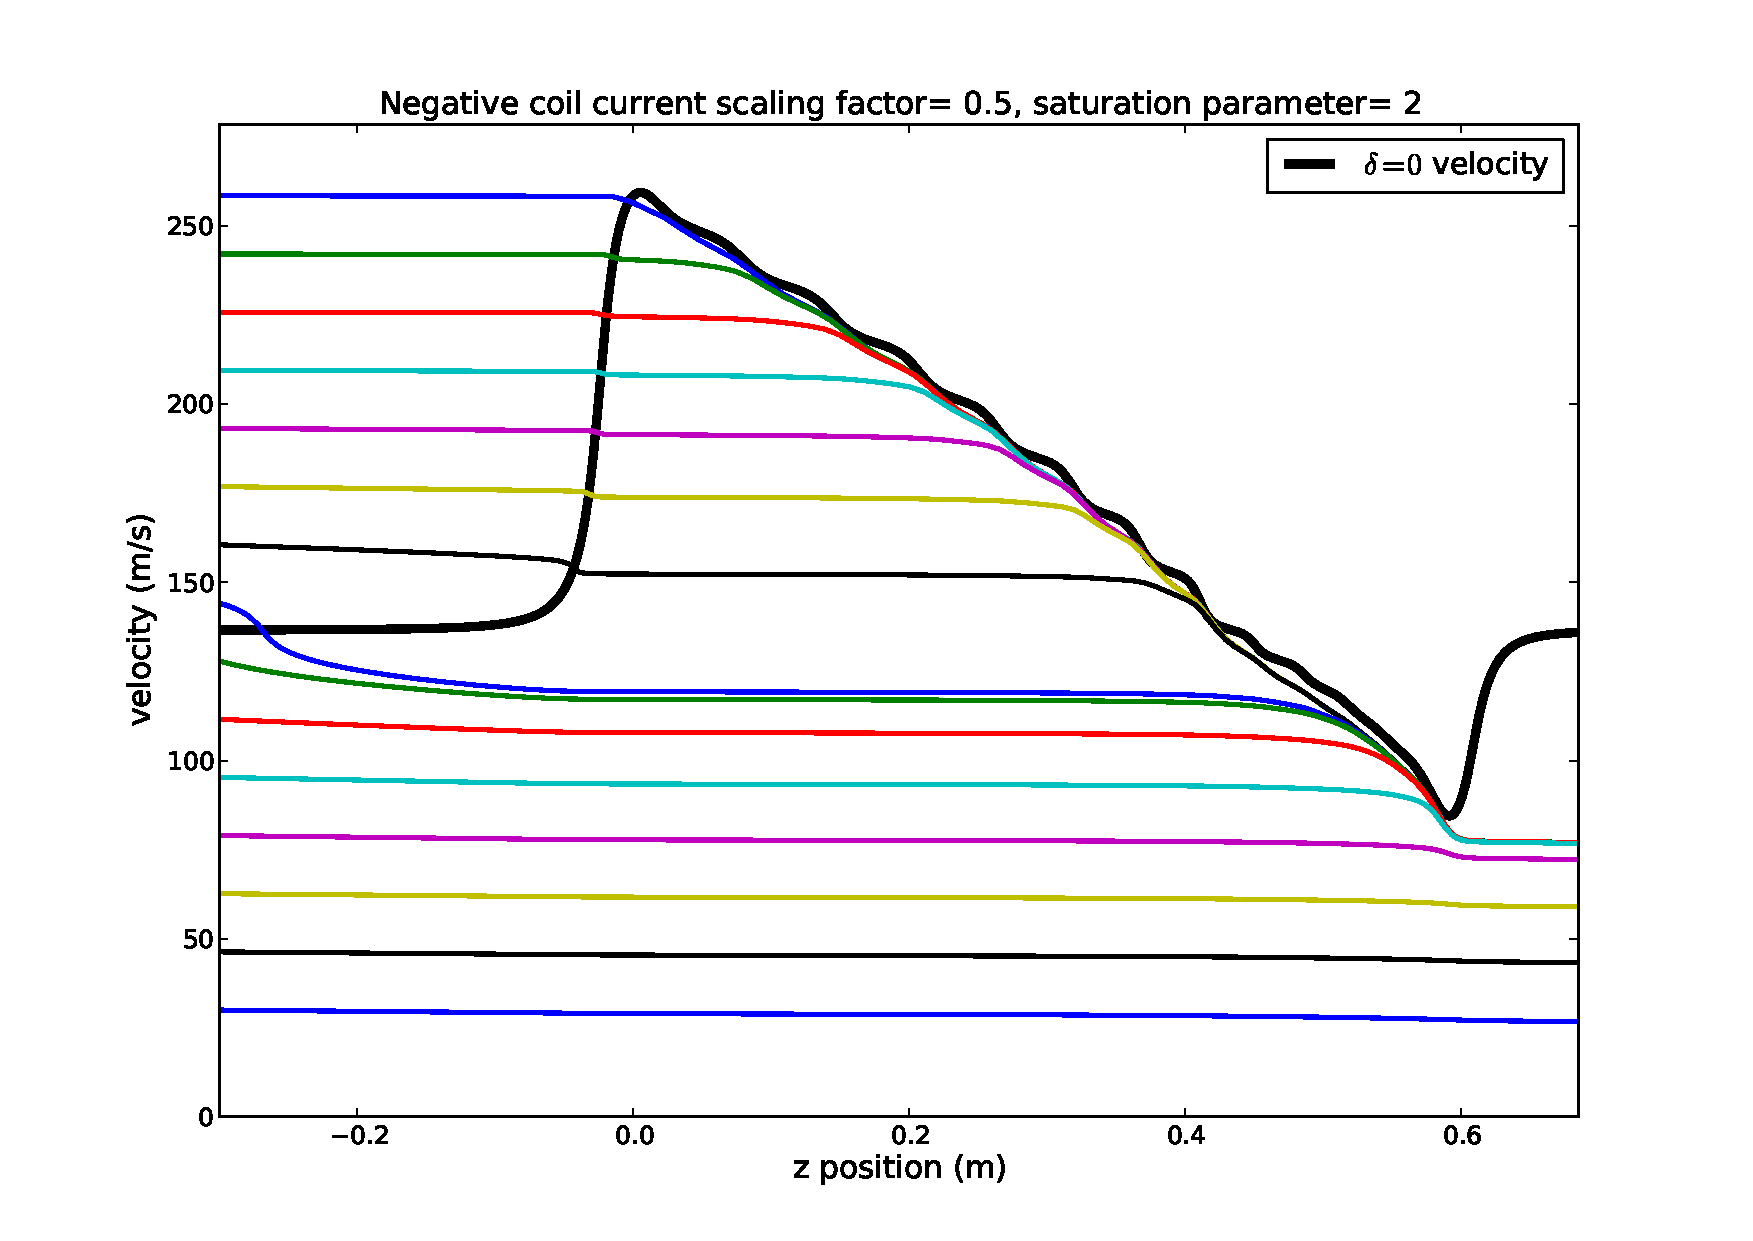
\includegraphics[width=0.9\textwidth]{trajectory03_2}
\caption{As Figure \ref{fig:trajectory1}, with reduced current in negative coil by a ratio of 0.5.}
\label{fig:trajectory2}
\end{figure}

\begin{figure}[htb]
\centering
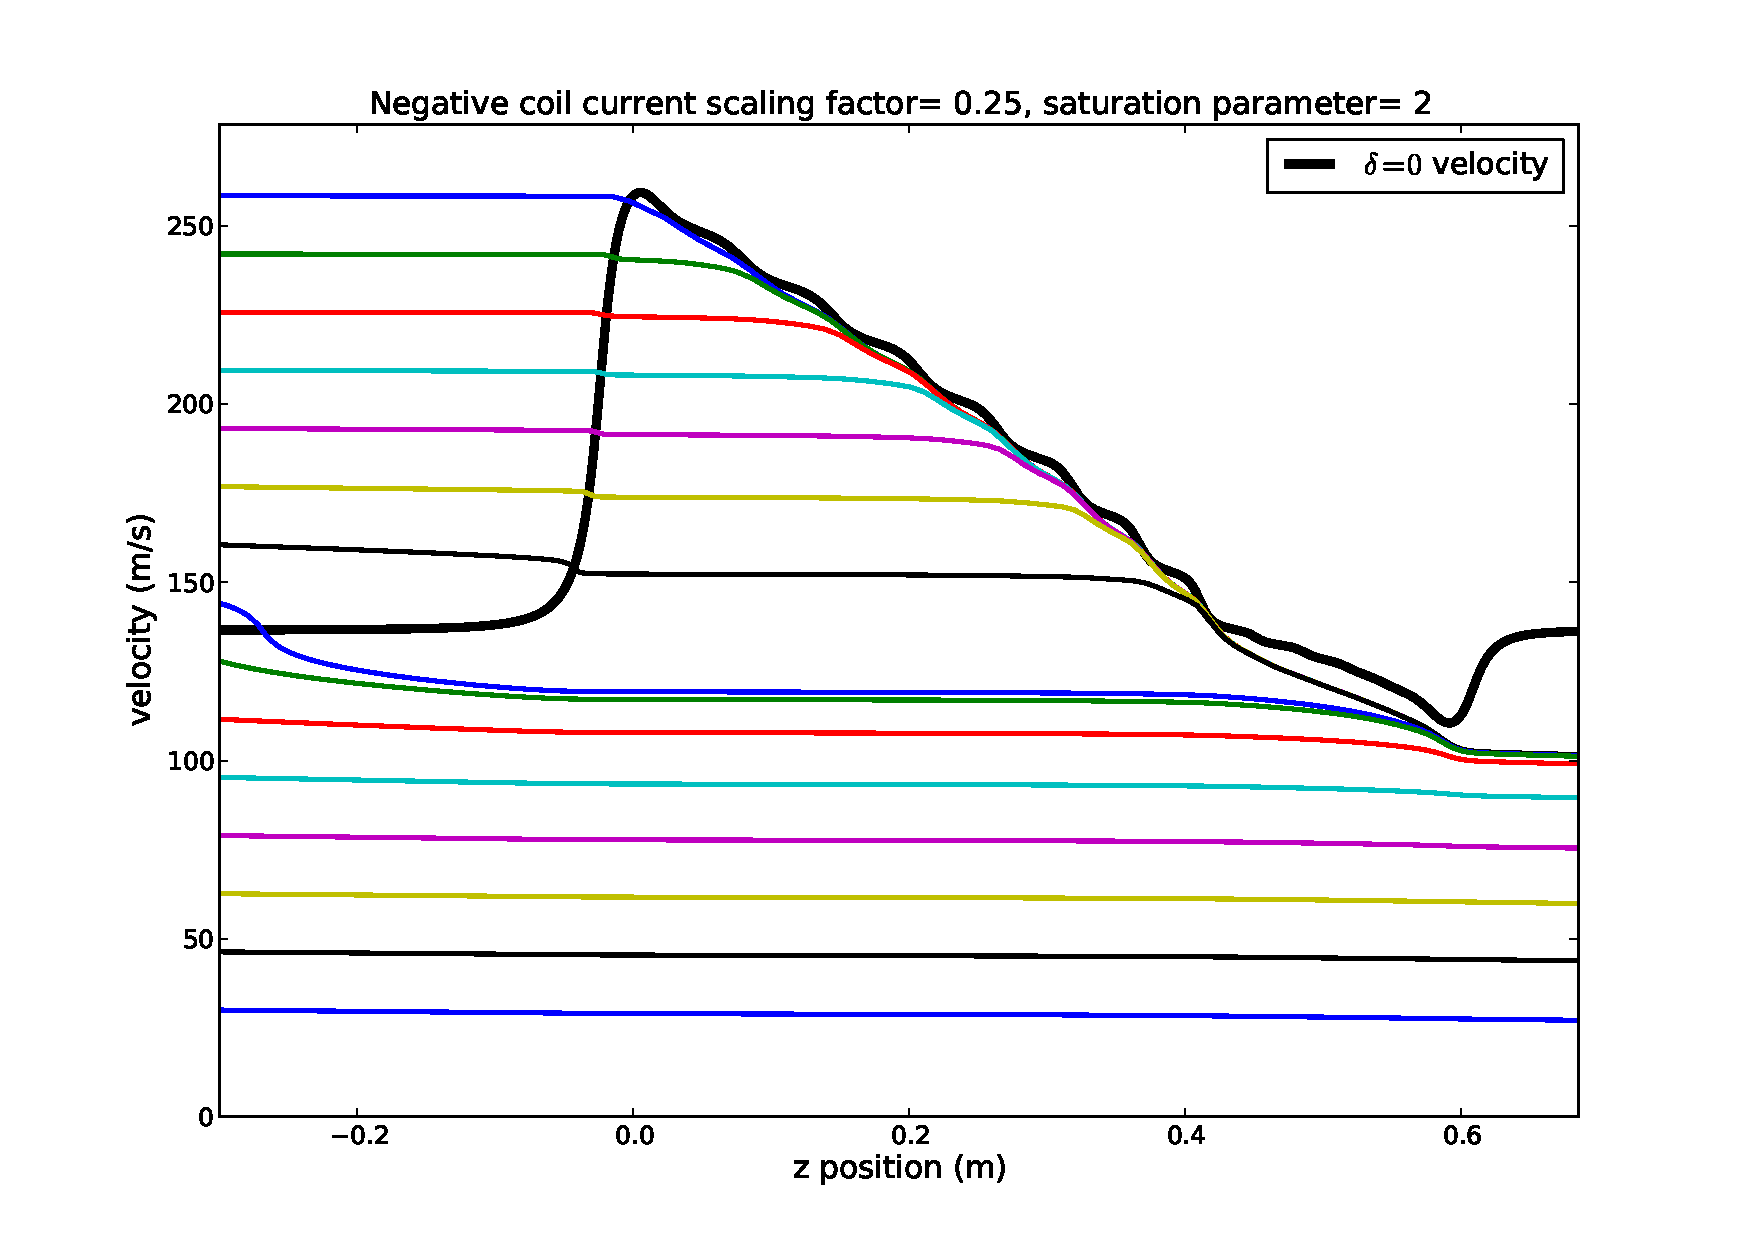
\includegraphics[width=0.9\textwidth]{trajectory03_3}
\caption{As Figure \ref{fig:trajectory1}, with reduced current in negative coil by a ratio of 0.25.}
\label{fig:trajectory3}
\end{figure}

\subsection{Assembly}

The slower was assembled in the mechanical workshop, using a lathe to turn the tube while winding the coil on top of it. The winding was done horizontally, first winding the whole first layer, turning back, and winding the next layer while keeping the same handedness of the cooils. Lower layers are usually positioned quite close to the specifications, while the higher layers have more position and winding error (i.e. longer spread than designed). As long as the wires are packed as tight as practically possible, this does not affect the final field profile too much.

The wires are kept in place with kapton tape, applied generously between layers and all around the wires. Later might add some high temperature epoxy to keep the whole structure even more rigid and ensure long term stability.

The final assembly was tested by applying a fixed current and measuring the magnetic field inside the tube as a function of position. Measurements were done with a borrowed AlphaLab GM-2 Gaussmeter\footnote{\url{http://www.trifield.com/content/dc-gaussmeter-model-gm2/}}, and Figure \ref{fig:slowerfield} shows the results. For comparison the simulated field is also shown. The absolute size of the simulated field is given by the applied current, the horizontal position is by measuring the coil position, and thus no fitting has been performed. Also plotted the expected field based on the actual measured coil positions. The end of the zeeman slower tube is indicated by vertical lines. 


The magnetic field values at and beyond the ends of the slower, given by simulation, are listed in the following table:

\begin{center}
\begin{tabular}{|c|c|c|}
\hline 
Magnetic field (G) & Postive coil & Negative coil \\ 
\hline 
At end & 2.4 & -2.8 \\ 
\hline 
35mm away & 0.8 & -0.8 \\ 
\hline 
70mm away & 0.4 & -0.3 \\ 
\hline 
\end{tabular} 
\end{center}

\begin{figure}[htb]
\centering
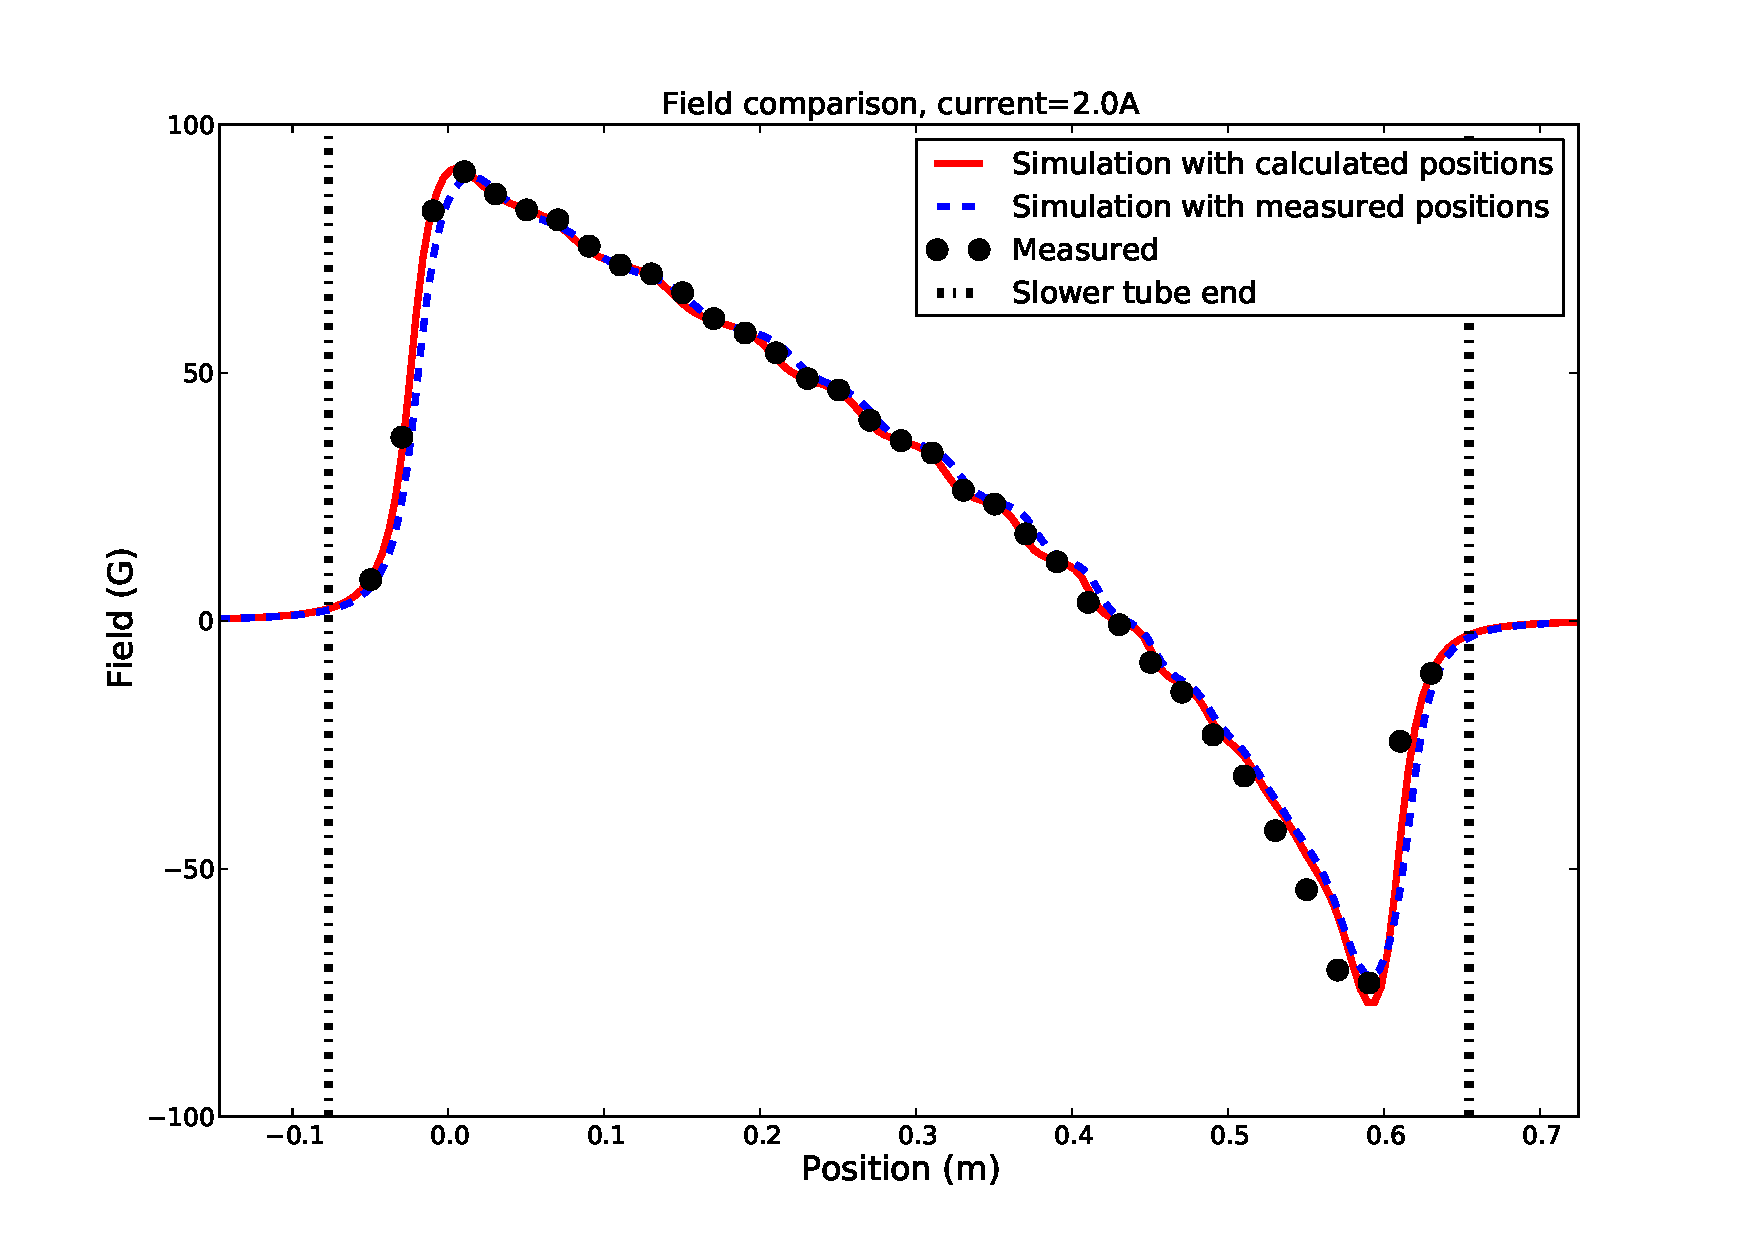
\includegraphics[width=0.9\textwidth]{slowerfield3}
\caption{The measured and simulated magnetic fields. They are in reasonable agreement, except for some positional uncertainty on the negative coil side. The ends of the Zeeman slower tube are indicated by vertical lines.}
\label{fig:slowerfield}
\end{figure}


\bibliographystyle{unsrt}
\bibliography{zeeman}
\end{document}